\documentclass[11pt]{article}
\usepackage[dvips]{graphics}
\usepackage{algorithmic}
\usepackage[ruled]{algorithm}
\usepackage{listings}
\usepackage{graphicx}
\usepackage{graphics}
\usepackage{array}
\usepackage{caption}
\usepackage{subfigure}
\usepackage{capt-of}
\usepackage{amsmath,amsfonts,amsthm} % Math packages
\newcommand{\tf}{{\hfill\fbox{{\large\bf True}}\qquad\fbox{{\large\bf False}}}}
\newcommand{\bfit}[1]{{\textbf{\textit{#1}}}}
\begin{document}
\lstset{language = c++, basicstyle=\footnotesize,breakatwhitespace=false,showstringspaces=false}
\title{Supervised Learning Project Report}
\author{GuiCheng Wu\\ Xinyi Xie}
\maketitle
%%%%%%%%%%%%%%%%%%%%%%%%%%%%%%%%%%%%%%%%%%%%%%%%%%%%%%%%%%%%%%%%%%%%%%%%
\section{Problem 1}
\subsection{KNN with k = 1,~5,~50}
The algorithm is very intuitive. For any test data $x_i$, we compute the distance between $x_i$ and all training data $\tilde{x}$ and store these distance into an array $A$, and sort array $A$ in an ascending order. For different $k$, we get the first $k$ element from array $A$ and their corresponding label. The majority label decides the label of our test data $x_i$.\\

We implement the KNN algorithm in both Matlab and Java. The file name of  the k-nearest neighbor algorithm is "knnForDigit.m". The test file of  the k-nearest neighbor algorithm is "testknnForDigit.m". We use 3437 instances in the dataset to train the knn model, and use 1000 instances to test the model.  The test results are as follows \\
When k = 1, the correct rate is 99.3\%. \\
When k = 5, the correct rate is 98.1\%. \\
When k = 50, the correct rate is 92.2\%.

\subsection{Support vector machine}
From the class, we learned that the soft-margin support vector machine has a prime problem as follows:
\begin{equation}
\begin{aligned}
\min_{\beta,\beta_0}&\frac{1}{2}||\beta||+C\sum_{i=1}^{N}\xi_i\\
\textrm{subject~to~}y_i&(x_i^T\beta+\beta_0)\ge1-\xi_i,~\xi_i\ge0,~i=1,...,N
\end{aligned}
\end{equation}
and its dual
\begin{equation}
\begin{aligned}
\min L_D &= \frac{1}{2}\sum_{i=1}^N\sum_{j=1}^N\alpha_i\alpha_j y_iy_jx_i^Tx_j^T-\sum_{i=1}^N\alpha_i\\
\textrm{subject~to~} &0 \le\alpha_i\leq C\\
\sum_{i=1}^N&\alpha_iy_i=0
\end{aligned}
\end{equation}
We use Matlab quadratical problem solver 'quadprog' to solve dual problem and the problem is formalized as follows to plug into 'quadprog'.
\begin{equation}
\begin{aligned}
\min L_D &= \frac{1}{2}\alpha^TH\alpha-f^T\alpha\\
\textrm{subject~to~} &A\alpha \le \textbf{C}\\
Aeq\alpha &= beq
\end{aligned}
\end{equation}
where $\alpha = (\alpha_1,...,\alpha_N)^T, H(i,j) = y_iy_jx_i^Tx_j^T,H\in N*N , f = (1,...,1)^T, A = \textrm{diag}(1,...,1)\in N*N, Aeq = (y_1,...,y_N)^T, beq = 0\in N*1$. And also $\alpha$ has lower bound 0 and upper bound C. Then we use  matlab command 'quadprog(H,f,A,b,Aeq,beq,LB,UB)' to solve $\alpha_i$ and then solve $\beta$ and $\beta_0$ using
\begin{equation}
\begin{aligned}
\beta &= \sum_{i=1}^N\alpha_iy_ix_i\\
\alpha_i(y_i(x_i^T\beta &+ \beta_0)-(1-\xi_i))=0.
\end{aligned}
\end{equation}
We also use an average of all the solutions for $\beta_0$ due to numerical stability. Since we have ten digit to classify, we build ten decision function to decide which digit our tests fall. Thus we have ten different $\alpha$ vectors, denoted by  $\alpha_{iR}$ which lead to ten different $\beta_{iR}$ and $\beta_{0iR}, i = 0,...,9$.
\begin{equation}
\begin{aligned}
f_{0R} &= x^T\beta_{0R}+\beta_{00R}\\
f_{1R} &= x^T\beta_{1R}+\beta_{01R}\\
f_{2R} &= x^T\beta_{2R}+\beta_{02R}\\
f_{3R} &= x^T\beta_{3R}+\beta_{03R}\\
f_{4R} &= x^T\beta_{4R}+\beta_{04R}\\
f_{5R} &= x^T\beta_{5R}+\beta_{05R}\\
f_{6R} &= x^T\beta_{6R}+\beta_{06R}\\
f_{7R} &= x^T\beta_{7R}+\beta_{07R}\\
f_{8R} &= x^T\beta_{8R}+\beta_{08R}\\
f_{9R} &= x^T\beta_{9R}+\beta_{09R}
\end{aligned}
\end{equation}
And the maximal of $f_{iR}$ decides the digit of the test $x$.\\
The file name of the support vector machine algorithm is "SVMDigitClassifier\_1.m". The test file of  the support vector machine algorithm is "TestSVMClassifier\_1.m". We implement three different kernels. They are implemented separately in the "GKernel.m", "DegreePolyKernel.m" and "NeuralNetworkKernel.m" files. Their equations are as follows\\
\begin{equation}
\textrm{Gaussian }: K(x, x') = exp(-|x - x'|^2/2\sigma^2);
\end{equation}
\begin{equation}
\textrm{polynomial} : K(x, x') = (1 + <x, x'>)^d;
\end{equation}
\begin{equation}
\textrm{neural ~network} : K(x, x') = tanh (k_1<x, x'> + k_2);
\end{equation}
where $<x,x'> = x^T*x'$.
And the process of solving kernel SVM  is a little different from original SVM. Instead of solving $\beta$, we solve kernel function. The other process are the same of original SVM. For the result of kernel SVM and original SVM, please check Problem 4.
\section{Problem 2}
The step for ten-fold cross validation: first, we choose $10\%$ of the train data randomly by using 'randsample'; then, the remaining $90\%$ of the data are used for training data while this $10\%$ are used for testing; finally, we run ten times and get an average confusion matrix. We have generated confusion matrix for knn, $k = 1, k = 5$, and $k= 50$.  And row $i$ and column $j$ means that the true label for this digit is $i$ and our algorithm predicts it as $j$. Therefore, it is a diagonally dominate matrix and exactly what we get. \\

$C_1$ is the confusion matrix computed by KNN for k = 1 and mean error is 0.64\%:

$$C_1 = \left(\begin{array}{cccccccccc} \frac{131}{1250} & 0 & 0 & 0 & \frac{1}{1250} & 0 & 0 & 0 & 0 & 0\\ 0 & \frac{188}{1875} & \frac{1}{1250} & 0 & 0 & 0 & 0 & 0 & 0 & 0\\ 0 & \frac{1}{750} & \frac{131}{1250} & 0 & 0 & 0 & 0 & 0 & 0 & 0\\ 0 & \frac{1}{3750} & 0 & \frac{121}{1250} & 0 & 0 & 0 & \frac{1}{1875} & 0 & 0\\ 0 & 0 & 0 & 0 & \frac{383}{3750} & 0 & 0 & 0 & 0 & \frac{1}{3750}\\ 0 & 0 & 0 & 0 & 0 & \frac{191}{1875} & 0 & 0 & 0 & 0\\ 0 & 0 & 0 & 0 & 0 & 0 & \frac{373}{3750} & 0 & 0 & 0\\ 0 & \frac{1}{1875} & 0 & \frac{1}{3750} & 0 & 0 & 0 & \frac{373}{3750} & 0 & 0\\ \frac{1}{3750} & 0 & 0 & 0 & 0 & 0 & 0 & 0 & \frac{341}{3750} & 0\\ 0 & \frac{1}{1875} & 0 & \frac{1}{3750} & \frac{1}{3750} & \frac{1}{3750} & 0 & 0 & 0 & \frac{349}{3750} \end{array}\right).$$

$C_2$ is the confusion matrix computed by KNN for k = 5 and mean error is 0.83\%:

 $$C_2 = \left(\begin{array}{cccccccccc} \frac{41}{375} & 0 & 0 & 0 & 0 & 0 & 0 & 0 & 0 & 0\\ 0 & \frac{383}{3750} & \frac{3}{1250} & \frac{4}{1875} & 0 & 0 & 0 & \frac{1}{3750} & 0 & 0\\ 0 & 0 & \frac{187}{1875} & 0 & 0 & 0 & 0 & 0 & 0 & 0\\ 0 & \frac{1}{3750} & \frac{1}{3750} & \frac{347}{3750} & 0 & \frac{1}{3750} & 0 & \frac{1}{3750} & 0 & 0\\ 0 & 0 & 0 & 0 & \frac{13}{125} & 0 & 0 & \frac{1}{3750} & 0 & 0\\ 0 & 0 & 0 & 0 & 0 & \frac{188}{1875} & 0 & 0 & 0 & 0\\ 0 & 0 & 0 & 0 & 0 & 0 & \frac{121}{1250} & 0 & 0 & 0\\ 0 & \frac{1}{1875} & 0 & 0 & 0 & 0 & 0 & \frac{181}{1875} & 0 & 0\\ \frac{1}{1250} & 0 & 0 & 0 & 0 & 0 & 0 & \frac{1}{3750} & \frac{182}{1875} & 0\\ 0 & 0 & 0 & \frac{1}{1875} & 0 & 0 & 0 & 0 & 0 & \frac{7}{75} \end{array}\right).
$$

$C_3$ is the confusion matrix computed by KNN for k = 50 and mean error is 6.43\%:
$$C_3 = \left(\begin{array}{cccccccccc} \frac{377}{3750} & 0 & 0 & 0 & \frac{3}{1250} & 0 & \frac{1}{625} & 0 & 0 & 0\\ 0 & \frac{107}{1250} & \frac{2}{125} & \frac{7}{1875} & 0 & \frac{1}{1875} & \frac{1}{1875} & \frac{7}{3750} & 0 & 0\\ 0 & \frac{1}{1250} & \frac{123}{1250} & 0 & 0 & 0 & 0 & 0 & 0 & 0\\ 0 & \frac{1}{625} & \frac{1}{1875} & \frac{61}{625} & 0 & 0 & 0 & \frac{1}{1250} & 0 & 0\\ 0 & \frac{1}{1875} & 0 & 0 & \frac{64}{625} & 0 & 0 & \frac{1}{1875} & 0 & 0\\ 0 & 0 & 0 & \frac{3}{1250} & 0 & \frac{178}{1875} & 0 & 0 & 0 & 0\\ 0 & 0 & 0 & 0 & 0 & 0 & \frac{176}{1875} & 0 & 0 & 0\\ 0 & \frac{13}{3750} & 0 & \frac{13}{3750} & 0 & 0 & 0 & \frac{347}{3750} & 0 & 0\\ \frac{1}{1250} & \frac{1}{625} & \frac{1}{1875} & \frac{7}{3750} & 0 & \frac{1}{750} & \frac{1}{750} & \frac{1}{375} & \frac{323}{3750} & \frac{1}{1250}\\ \frac{1}{625} & \frac{11}{3750} & 0 & \frac{3}{1250} & \frac{2}{1875} & \frac{17}{3750} & 0 & 0 & 0 & \frac{157}{1875} \end{array}\right).$$
We only computer SVM using Gaussian kernel with $C=0.05$ and $\sigma = 59$ due to the huge amount of time. Mean error is 4.55\%.
$$
C_4 = \left(\begin{array}{cccccccccc}
0.1093&0.0107&0     &0     &0     &0     &0     &0     &0     &0      \\
0     &0.1147&0.0080&0.0027&0     &0     &0     &0     &0     &0      \\
0     &0.0053&0.1200&0     &0     &0     &0     &0     &0     &0      \\
0     &0     &0     &0.0960&0     &0     &0     &0     &0     &0      \\
0     &0.0027&0     &0     &0.0960&0     &0     &0     &0     &0.0027 \\
0     &0     &0     &0     &0     &0.0933&0     &0     &0     &0.0027 \\
0     &0     &0     &0     &0     &0     &0.0693&0     &0     &0      \\
0     &0     &0     &0     &0     &0     &0     &0.0827&0     &0      \\
0     &0.0053&0     &0     &0     &0     &0     &0     &0.0827&0      \\
0     &0.0027&0     &0     &0     &0.0027&0     &0     &0     &0.0907 \\
\end{array}\right).$$
\section{Problem 3}
For Guassian SVM formulation, we have each digit as follows. We use train data and the error is less than $0.05$, $|f_{iR} - 1| \le 0.05 $. Please check (Figure 1) and (Figure 2).
\begin{figure}[htbp]
\begin{center}
\subfigure[digit 0]{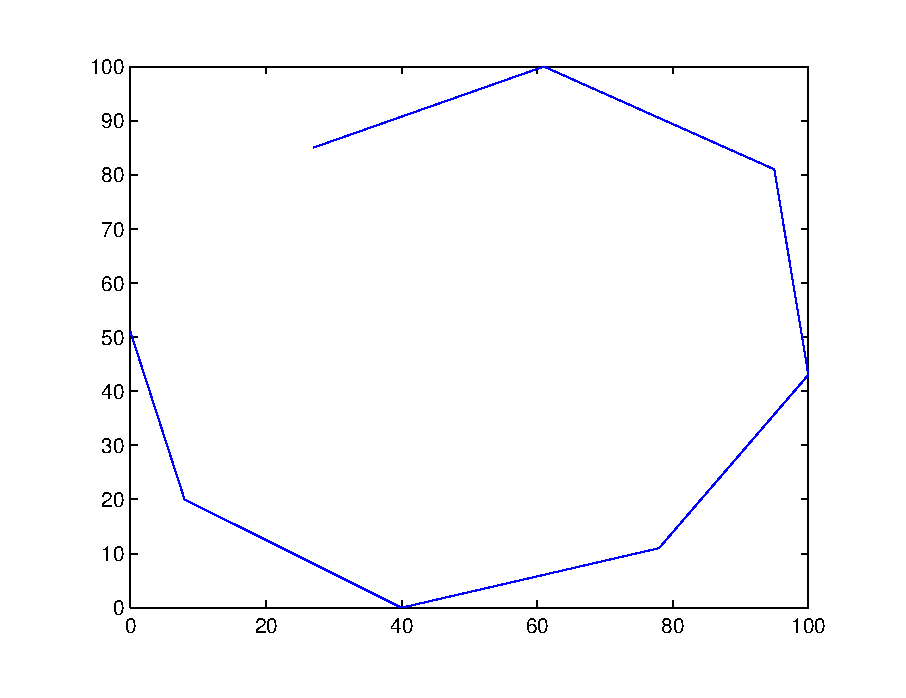
\includegraphics[width=2in]{0_14.eps}}
\subfigure[digit 1]{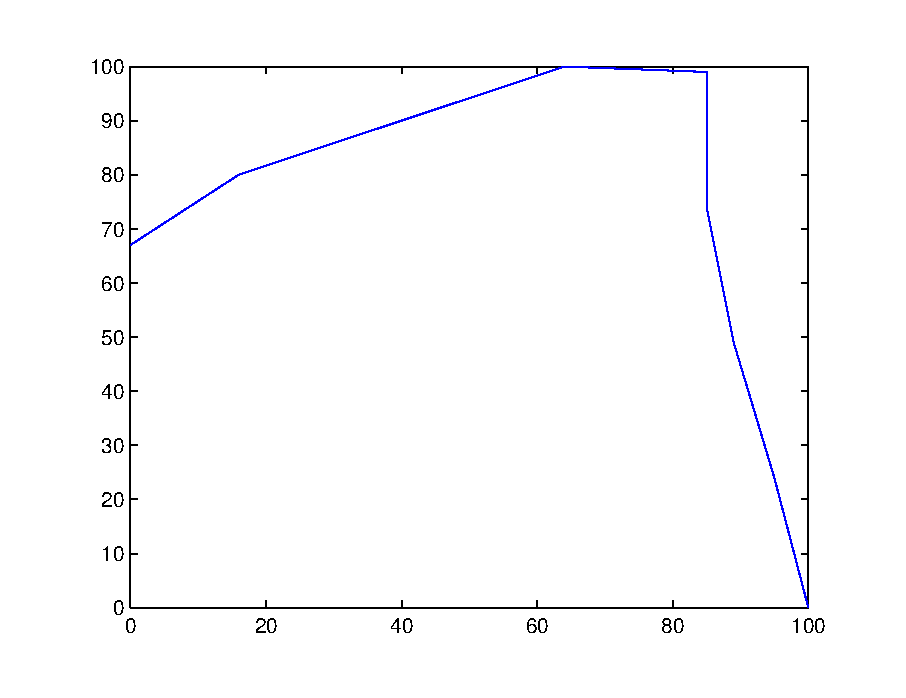
\includegraphics[width=2in]{1_409.eps}}
\subfigure[digit 2]{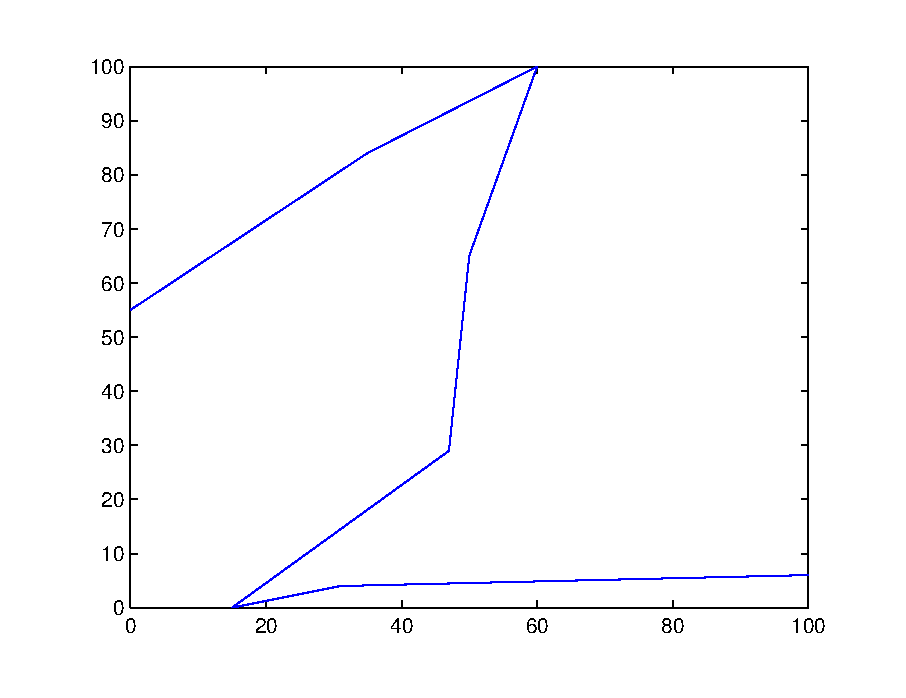
\includegraphics[width=2in]{2_591.eps}}
\subfigure[digit 3]{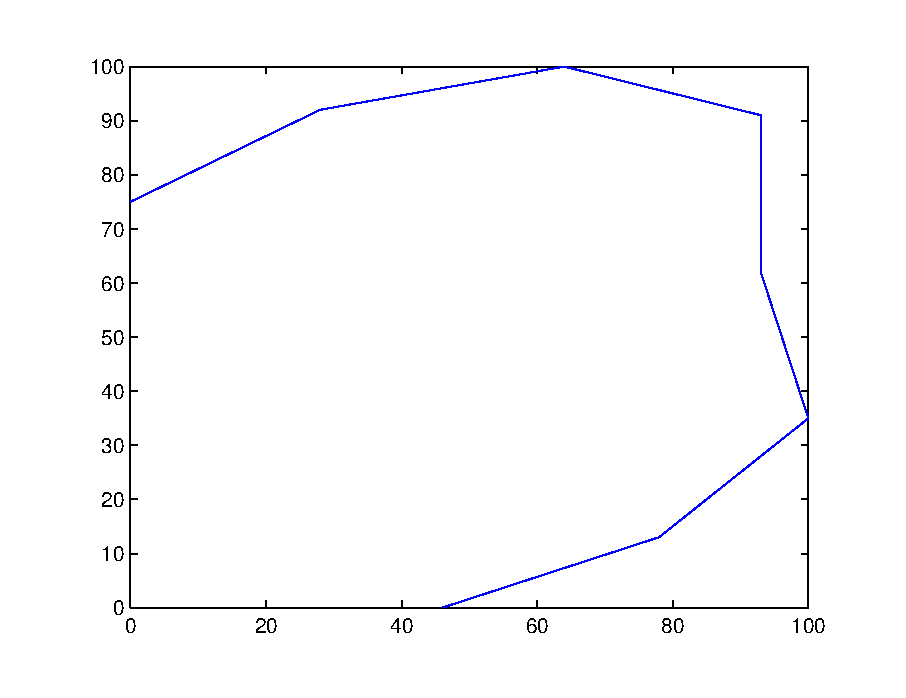
\includegraphics[width=2in]{3_1228.eps}}
\subfigure[digit 4]{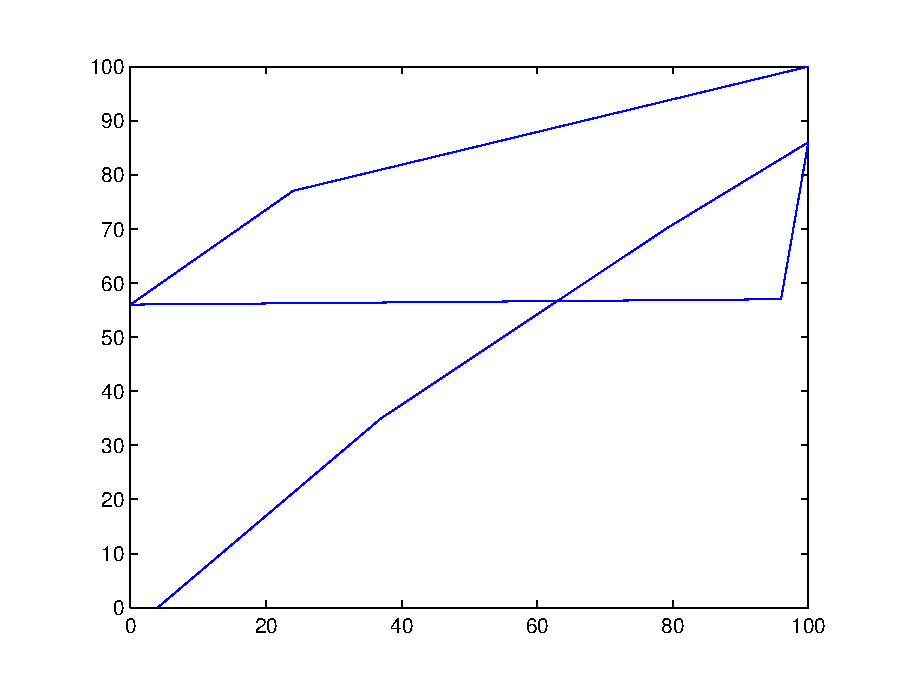
\includegraphics[width=2in]{4_1538.eps}}
\subfigure[digit 5]{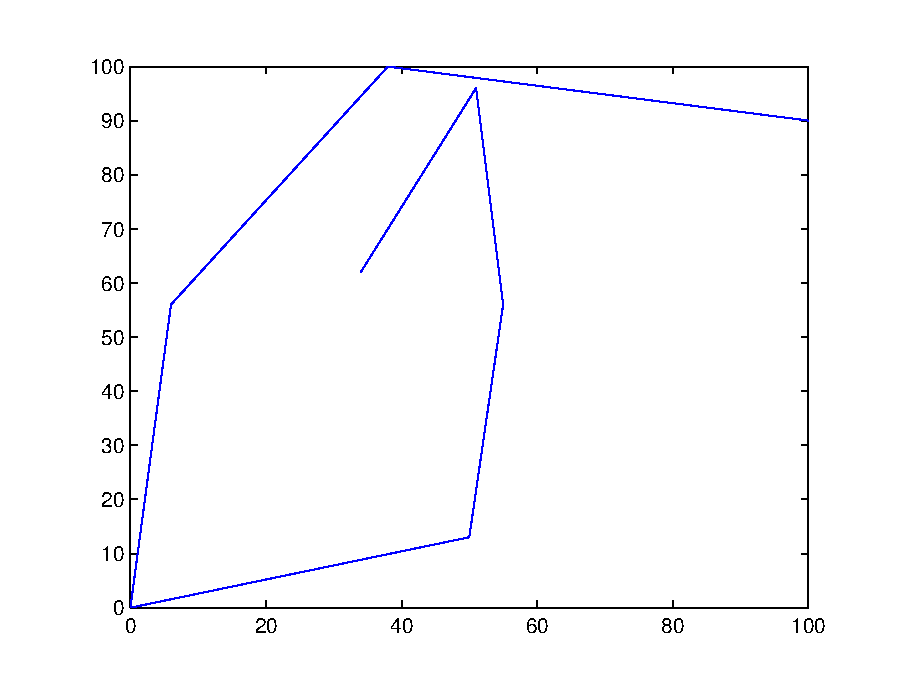
\includegraphics[width=2in]{5_2163.eps}}
\subfigure[digit 6]{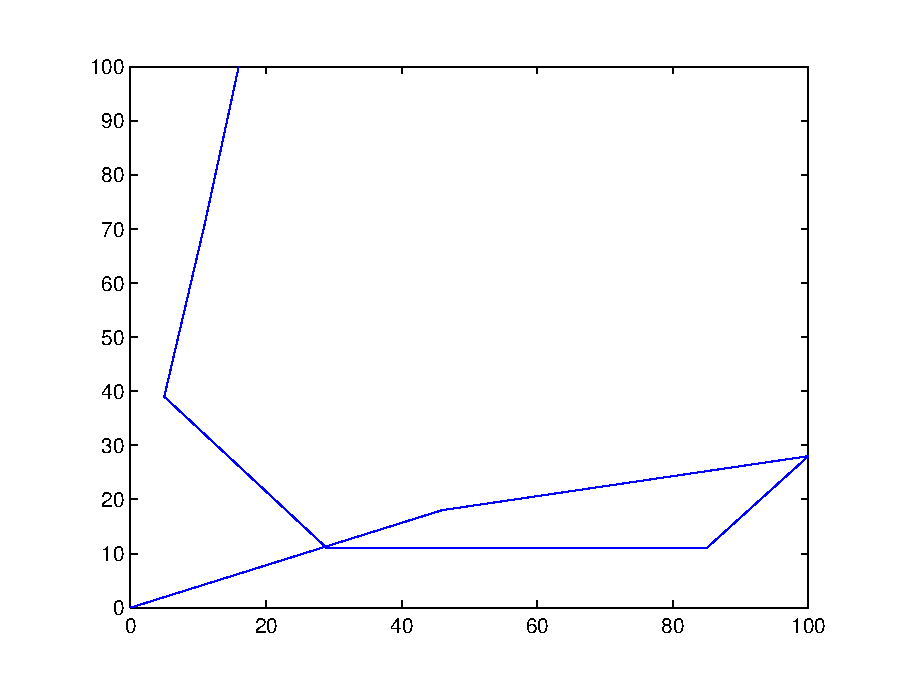
\includegraphics[width=2in]{6_2473.eps}}
\subfigure[digit 7]{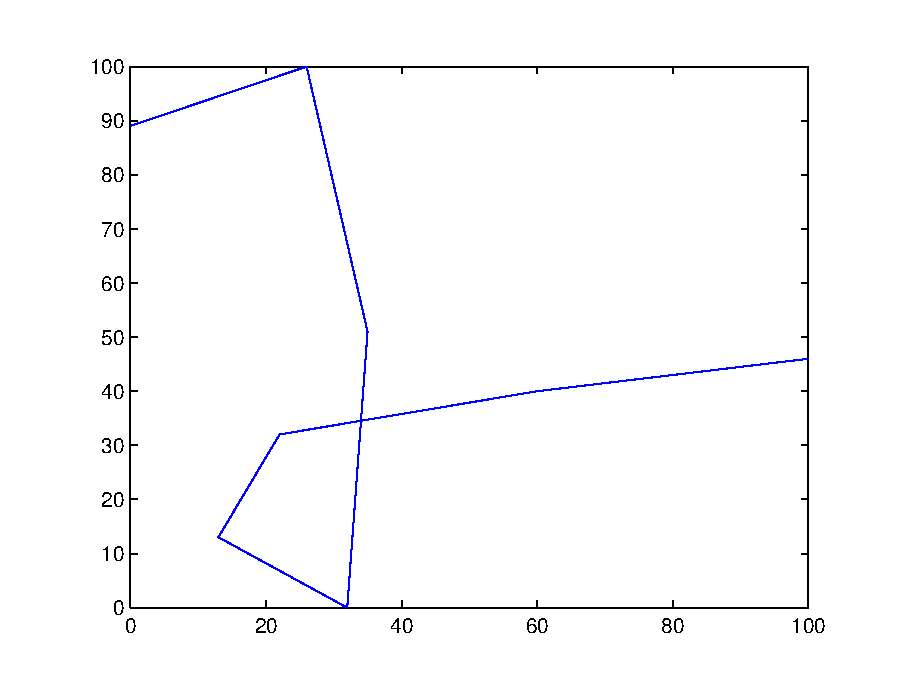
\includegraphics[width=2in]{7_2744.eps}}
\caption{These figures present the support vector for digit 0 to 7}
\end{center}\label{figure1}
\end{figure}
\begin{figure}[htbp]
\begin{center}
\subfigure[digit 8]{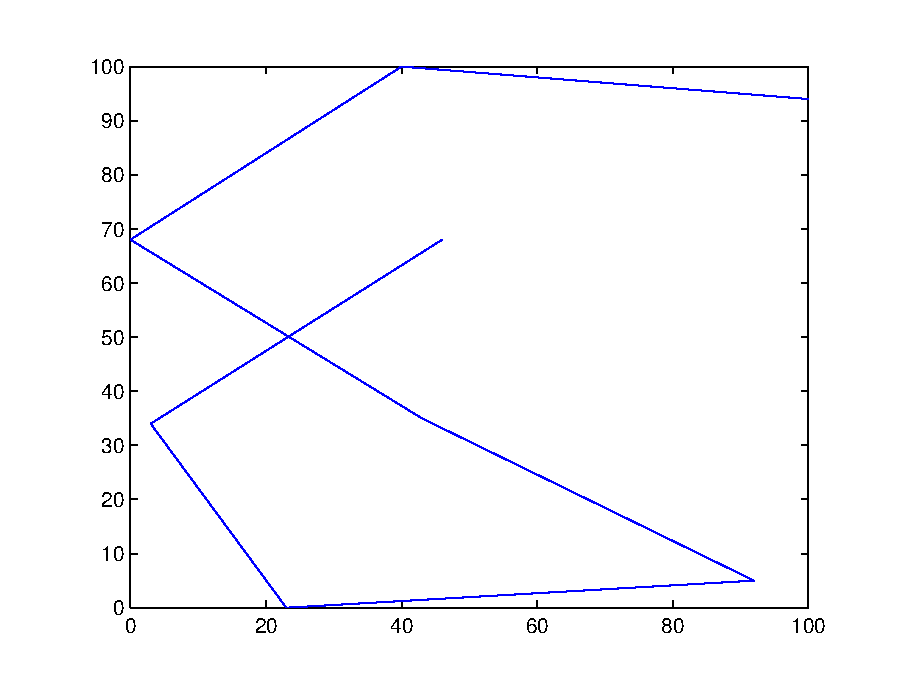
\includegraphics[width=2in]{8_3040.eps}}
\subfigure[digit 9]{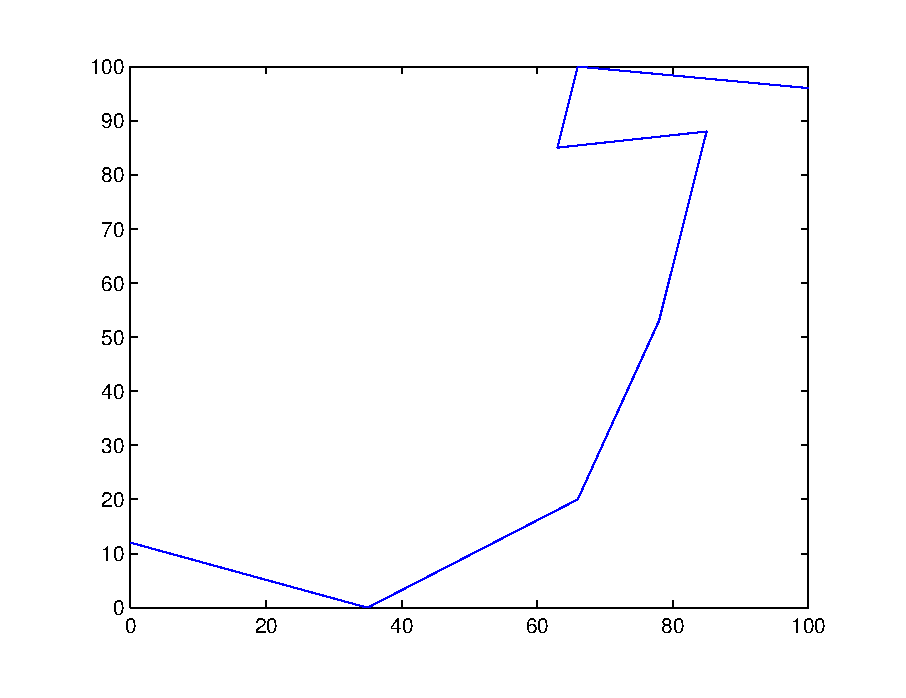
\includegraphics[width=2in]{9_3392.eps}}
\caption{These figures present support vector for 8 and 9}
\end{center}\label{figure2}
\end{figure}

\section{Problem 4}
SVM is beneficial from generalization power because it is capable of moving the entire problem into a representation of greater dimension, enabling it to separate more complex problems. While KNN method is very intuitive, it computes the similarity of two digits and using majority vote to decide which label it is.\\
The following table gives the overall correct rate of our methods. And as you can see, KNN-1 method has a very high correct rate because this problem is more like a local consistency problem.\\
\begin{tabular}{|c|c|c|}
  \hline
  % after \\: \hline or \cline{col1-col2} \cline{col3-col4} ...
  \textrm{label} & \textrm{Correct Rate} &\textrm{Parameter}\\ \cline{1-3}
  \textrm{KNN-1} & 99.3\% & $k = 1$ \\
  \textrm{KNN-5} & 98.1\% &$k=5$\\
  \textrm{kNN}-50 & 92.2\% &$k=50$\\
  \textrm{SVM} & 99\%  & $C=0.05, \xi = 5e-5$\\
  \textrm{SVM-Gaussian} & 96.4\% & $C= 0.05,\sigma = 59$\\
  \textrm{SVM-Polynomial} & 98.4\% & $C= 0.05, d = 4$\\
  \textrm{SVM-Neural Network} & 87.03\%& $C=0.05,k_1=0.2,k_2=-2$\\
  \hline
\end{tabular}
\\

We also compare the SVM and 1NN method for every digit by using the confusion matrix in the problem 2. As we can see,  1NN predict some 9 as 1 and SVM does not. SVM predict some 5 to 10 and 1NN does not. This is because KNN is local consistency and SVM is global consistency. If it is global consistency, it can be separated by a hyperplane. When it is local consistency, majority vote is very efficient.
\section{Problem 5}
We predict the digit using KNN-1 algorithm, the result is in the "3\_predictResult.csv" file.
\section{Problem 6}
The transfer SVM algorithm is  in the "TransferSVM.m" file. The algorithm is as follows. First, solve source data set and get solution of $\beta_s$ and $\beta_{s0}$. Then solve the dual problem of target set and get solution of $\beta_{t}$. After that, we solve $\beta_{t0}$ using equation
\begin{equation}
\alpha_{i}(y_i(x_i^T\beta_s + \beta_{s0}) + y_i(x_i^T\beta_t + \beta_{t0})) = 1 - \xi_i
\end{equation}
where we already solved $\beta_s, \beta_{s0}$ and $\beta_t$. Finally, we compute the $f_{08}$ like $f_{iR}$ in the problem 1. And when $f_{08} \ge 0$, we label the digit as 0. When $f_{08} < 0$, we label the digit as 8.
The result is in the "6\_0vs8TestResult.csv" file.
\section{Code}
All the codes are inside the "code" folder.
\end{document}


